\documentclass[tikz,border=3.14mm]{standalone}
\usepackage{pgfplots}
\pgfplotsset{compat=1.16}
\begin{document}
    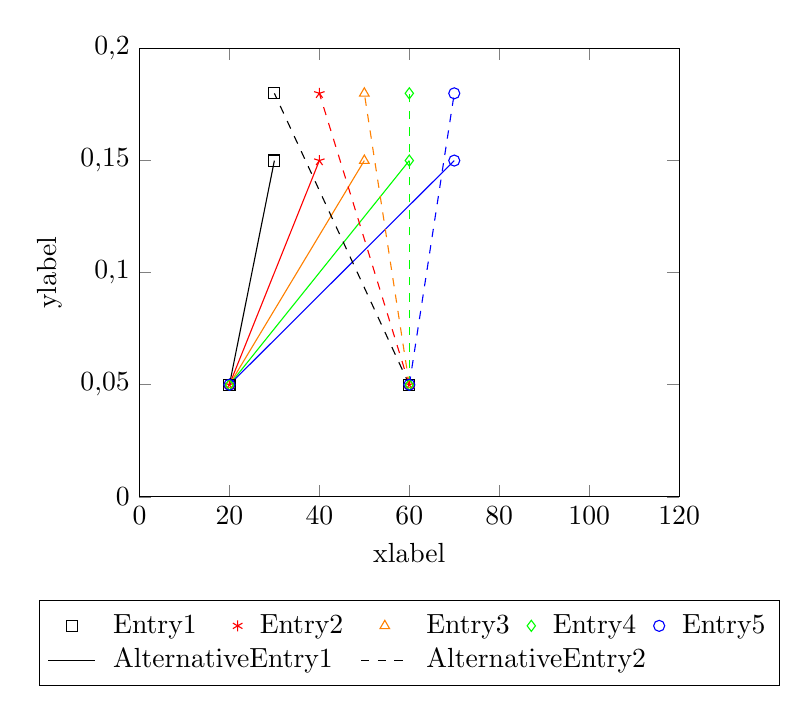
\begin{tikzpicture}
    \begin{axis}
    [
    ylabel={ylabel}, 
    xlabel={xlabel},  
    xmin=0, 
    xmax=120, 
    ymin=0, 
    ymax=0.2,
    legend columns = 5,
    legend style = {at={(0.5, -0.23)}, anchor=north, inner sep=3pt, style={column sep=0.15cm}},       %vorher: at={(1.3, 1)}
    legend cell align=left,
    ticklabel style={
        /pgf/number format/.cd,
        fixed,
        use comma,
    }
    ]


    \addlegendimage{black, only marks, mark=square} % or mark=none?
    \addlegendentry{Entry1}

    \addlegendimage{red, only marks, mark=asterisk}
    \addlegendentry{Entry2}

    \addlegendimage{orange, only marks, mark=triangle}
    \addlegendentry{Entry3}

    \addlegendimage{green, only marks, mark=diamond}
    \addlegendentry{Entry4}

    \addlegendimage{blue, only marks, mark=o}
    \addlegendentry{Entry5}

    \addlegendimage{black, line legend}
    \addlegendentry{\makebox[0pt][l]{AlternativeEntry1}}

    \addlegendimage{empty legend}
    \addlegendentry{}
    \addlegendimage{black, line legend, dashed}
    \addlegendentry{\makebox[0pt][l]{AlternativeEntry2}}

    \addplot[color=black, mark=square] coordinates {(20,0.05)(30,0.15)};
    \addplot[color=red, mark=star] coordinates {(20,0.05)(40,0.15)};
    \addplot[color=orange, mark=triangle] coordinates {(20,0.05)(50,0.15)};
    \addplot[color=green, mark=diamond] coordinates {(20,0.05)(60,0.15)};
    \addplot[color=blue, mark=o] coordinates {(20,0.05)(70,0.15)};

    \addplot[color=black, mark=square, dashed, mark options={solid}] coordinates {(60,0.05)(30,0.18)};
    \addplot[color=red, mark=star, dashed, mark options={solid}] coordinates {(60,0.05)(40,0.18)};
    \addplot[color=orange, mark=triangle, dashed, mark options={solid}] coordinates {(60,0.05)(50,0.18)};
    \addplot[color=green, mark=diamond, dashed, mark options={solid}] coordinates {(60,0.05)(60,0.18)};
    \addplot[color=blue, mark=o, dashed, mark options={solid}] coordinates {(60,0.05)(70,0.18)};

    \end{axis}
    \end{tikzpicture}
\end{document}